\chapter{Implementation}
This chapter highlights the implementational aspects of the system. Introducing the technologies used to build the components. Each section is referring to its respective GitHub repository of the \texttt{ARTIS-project}\footnote{\href{https://github.com/artis-project/}{https://github.com/artis-project/}} GitHub organization.

\section{artis-rockpi-logger}

\begin{wrapfigure}[15]{o}{0.5\textwidth}
    \centering
    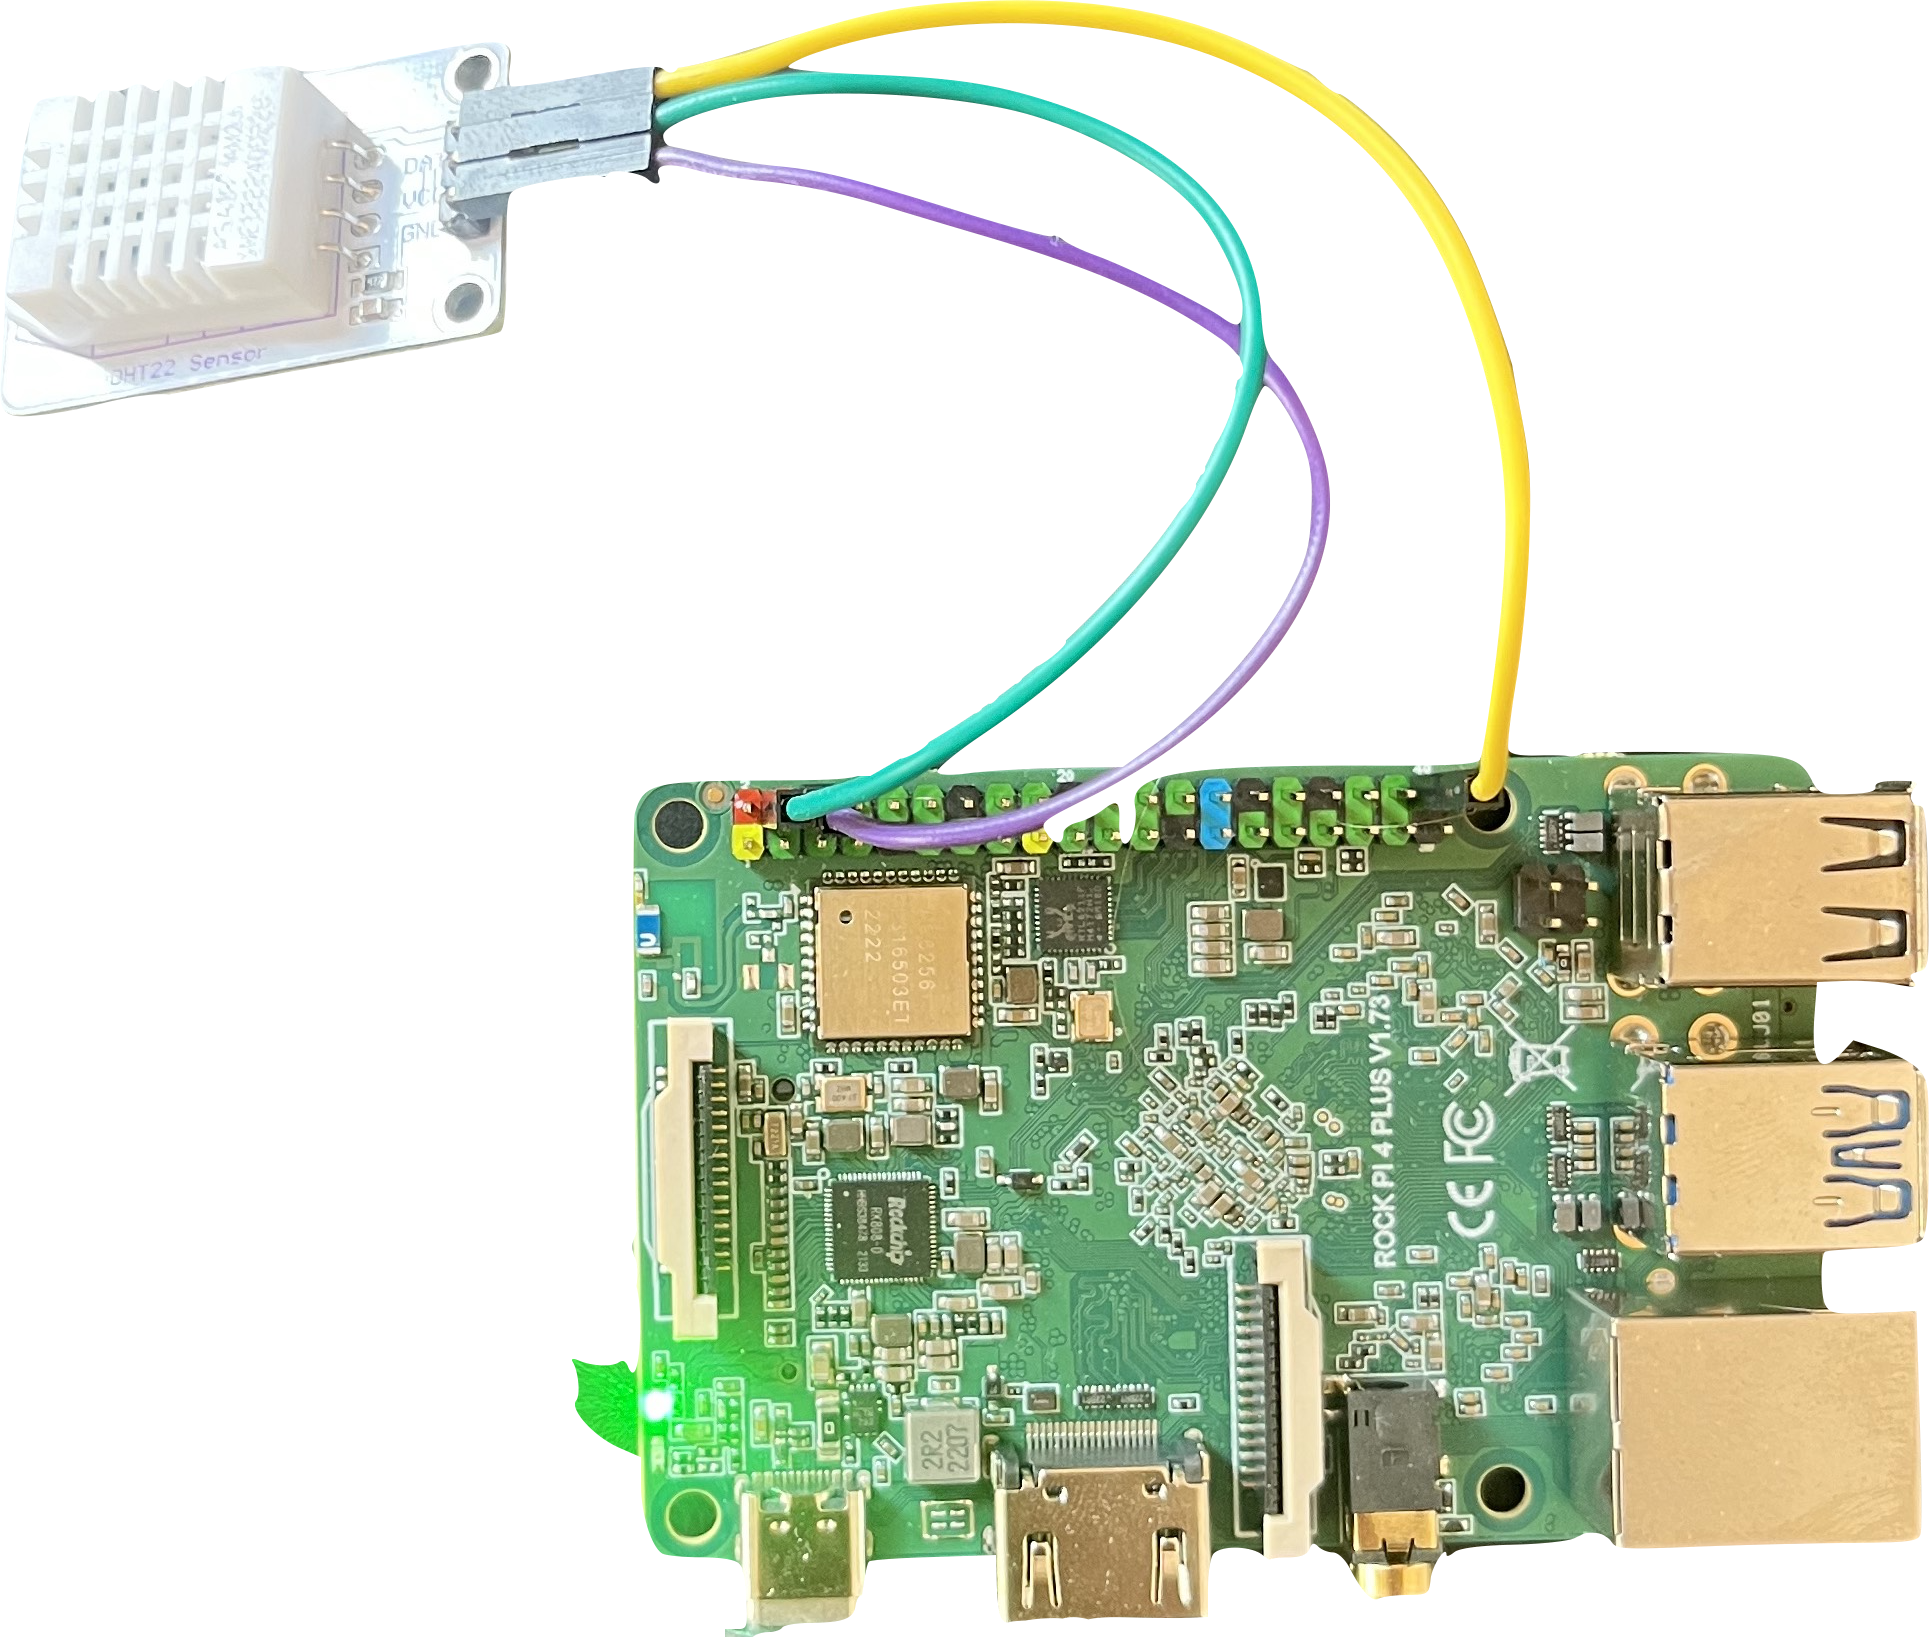
\includegraphics[width=0.49\textwidth]{resources/rock-pi.png}
    \caption{Rock Pi with a DHT-22 sensor} 
    \label{fig:rock-pi}
\end{wrapfigure}

For this project, we used a Rock Pi \footnote{\href{https://rockpi.org/rockpi4}{https://rockpi.org/rockpi4}} with a DHT-22\footnote{\href{https://www.adafruit.com/product/385}{https://www.adafruit.com/product/385}} sensor attached. (figure \ref{fig:rock-pi})

The decision for this device and sensor is based on simplicity and flexibility as well as on low acquisition costs. The Rock Pi is compatible with Linux operating systems which makes it very simple to write scripts using high-level programming languages like Python. It also has \gls{gpio} support to easily connect the DHT-22 sensor. The sensor is capable of recording temperature and humidity data from the environment.

\subsection{Sensor Interface}
\begin{wrapfigure}{O}{0.4\textwidth}
    \centering
    \begin{forest}
      for tree={
        font=\ttfamily,
        grow'=0,
        child anchor=west,
        parent anchor=south,
        anchor=west,
        calign=first,
        edge path={
          \noexpand\path [draw, \forestoption{edge}]
          (!u.south west) +(7.5pt,0) |- node[fill,inner sep=1.25pt] {} (.child anchor)\forestoption{edge label};
        },
        before typesetting nodes={
          if n=1
            {insert before={[,phantom]}}
            {}
        },
        fit=band,
        before computing xy={l=15pt},
      }
    [artis-rockpi-logger
      [/Rockfruit\_Python\_DHT
      ]
      [artis\_api.py
      ]
      [jwt.py
      ]
      [logging\_script.py
      ]
      [violation\_script.py
      ]
    ]
    \end{forest}
    \caption{Filetree of the artis-rockpi-logger repository}
    \label{fig:artis-logger-filetree}
\end{wrapfigure}
To read data from the DHT-22 sensor we used an existing library called Rockfruit\_Python\_DHT\footnote{\href{https://github.com/Tim-J-Parbs/Rockfruit_Python_DHT}{https://github.com/Tim-J-Parbs/Rockfruit\_Python\_DHT}}. The library provides a function with the signature \texttt{read\_retry(sensor, pin, retries=15, delay\_seconds=2)}. This method reads data from the DHT sensor of the specified type (in our case 22) on the specified \gls{gpio} pin and returns a tuple of humidity (as a floating point value in percent) and temperature (as a floating point value in Clesius). The function will attempt to read multiple times (up to the specified retries) until a reading can be registered. If no reading can be registered after the amount of retries the function will return \texttt{(None, None)}. The default delay between retries is two seconds, but can be overridden.

\section{artis-smartcontract}
The \gls{sc} was written in Ethereums native programming language Solidity \cite{solidity}. The contract was developed using hardhat \cite{hardhat}, a development environment for Ethereum. Hardhat makes it easy to develop, compile, test and deploy smartcontracts. The \gls{sc} has been deployed to the Ethereum Testnet Sepolia \cite{sepolia} during development, but is intended to be deployed on the Mainnet in production. 


A decentralized, distributed ledger that stores transactions or data in a secure, tamper-resistant, and tamper-evident fashion. The blockchain can be used to create and track \glspl{nft}, their ownership and provenance as well as the data associated with it. For this project we selected the Ethereum network due to prior experience of the research group and the author. 

The blockchain component consists of an Ethereum full-node that provides a \gls{rpc} endpoint and a \gls{sc}, which will be written in solidity. For simplicity, the project will take advantage of a managed full-node and not provide its own.


\section{artis-server}
